%% Los cap'itulos inician con \chapter{T'itulo}, estos aparecen numerados y
%% se incluyen en el 'indice general.
%%
%% Recuerda que aqu'i ya puedes escribir acentos como: 'a, 'e, 'i, etc.
%% La letra n con tilde es: 'n.
\chapter{Resultados}
\section{Paquete de R \emph{geneticae}}

El paquete \emph{geneticae} ofrece funciones para el análisis de datos de etapas avanzadas de programas de mejoramiento, donde se evalúan pocos genotipos. 

Para instalarlo se deben ejecutar las siguientes instrucciones:

\begin{lstlisting}
install.packages("devtools")
library(devtools)
install_github("jangelini/geneticae")
\end{lstlisting}

Una vez que se instala el paquete geneticae, se debe cargar en la sesion de R indicando:

\begin{lstlisting}
library(geneticae)
\end{lstlisting}


Es posible obtener información detallada sobre las funciones del paquete geneticae mediante de los archivos de ayuda indicando \emph{help (package = "geneticae")}.  La ayuda para una función, por ejemplo, \emph{imputation}, en una sesión R se puede obtener usando \emph{?imputation} o \emph{help(imputation)}.


\subsection{Conjuntos de datos en geneticae}

El paquete geneticae proporciona dos conjuntos de datos para ilustrar la metodología incluida para analizar los datos MET.

\begin{itemize}
\item yan.winterwheat dataset: rendimiento de 18 variedades de trigo de invierno cultivadas en nueve ambientes en Ontario en 1993. No hay réplicas disponibles en los datos. Este conjunto de datos se obtuvo del paquete agridat.
\end{itemize}
\begin{lstlisting}
library(geneticae)
data(yan.winterwheat)
dat_yan <- yan.winterwheat
head(dat_yan)
\end{lstlisting}

\begin{verbatim}
##   gen  env yield
## 1 Ann BH93 4.460
## 2 Ari BH93 4.417
## 3 Aug BH93 4.669
## 4 Cas BH93 4.732
## 5 Del BH93 4.390
## 6 Dia BH93 5.178
\end{verbatim}
\begin{itemize}
\item plrv dataset: rendimiento, peso de planta y parcela de 28 clones de la población del virus del enrollamiento de la papa (PLRV) evaluada en seis entornos. Las réplicas están disponibles en los datos. Este conjunto de datos se obtuvo del paquete agricolae.
\end{itemize}
\begin{lstlisting}
data(plrv)
dat_rep <- plrv
head(dat_rep)
\end{lstlisting}


\begin{verbatim}
##   Genotype Locality Rep WeightPlant WeightPlot    Yield
## 1   102.18     Ayac   1   0.5100000       5.10 18.88889
## 2   104.22     Ayac   1   0.3450000       2.76 12.77778
## 3   121.31     Ayac   1   0.5425000       4.34 20.09259
## 4   141.28     Ayac   1   0.9888889       8.90 36.62551
## 5   157.26     Ayac   1   0.6250000       5.00 23.14815
## 6    163.9     Ayac   1   0.5120000       2.56 18.96296
\end{verbatim}

 
\subsection{Funciones en geneticae}

\textbf{Modelo de regresión por sitio}

Para ejecutar la función \emph{GGEmodel}, se debe proporcionar un conjunto de datos con genotipos, ambientes, repeticiones (si hay disponibles), el fenotipo observado y los nombres que dichas variables tienen en el archivo de entrada. Además, se debe indicar el método de centrado, escala y SVD.

Cuando no hay repeticiones disponibles en el conjunto de datos, como es el caso del conjunto de datos yan.winterwheat, el modelo GGE se indica de la siguiente manera:


\begin{lstlisting}
GGE1 <- GGEmodel(dat_yan, genotype = "gen", environment = "env", 
response = "yield", centering = "tester")
\end{lstlisting}


Sin embargo, en el caso de que haya repeticiones disponibles, como el conjunto de datos plrv, se indica de la siguiente manera:


\begin{lstlisting}
GGE1_rep <- GGEmodel(dat_rep, genotype = "Genotype", environment = "Locality", 
response = "Yield", rep = "Rep", centering = "tester")
\end{lstlisting}


La salida de la función GGEmodel es una lista con los siguientes elementos:


\begin{itemize}
\item coordgenotype: trazado de coordenadas para genotipos de todos los componentes.
\item coordenviroment: trazado de coordenadas para entornos de todos los componentes.
\item valores propios: vector de valores propios de cada componente.
\item vartotal: varianza general.
\item varexpl: porcentaje de varianza explicado por cada componente.
\item labelgen: nombres de genotipo.
\item labelenv: nombres de entorno.
\item ejes: etiquetas de eje.
\item Datos: datos de entrada escalados y centrados.
\item centrado: nombre del método de centrado.
\item escala: nombre del método de escala.
\item SVP: nombre del método SVP.
\end{itemize}


Por ejemplo, para el conjunto de datos yan.winterwheat:


\begin{lstlisting}
names(GGE1)
\end{lstlisting}

\begin{verbatim}
##  [1] "coordgenotype"   "coordenviroment" "eigenvalues"    
##  [4] "vartotal"        "varexpl"         "labelgen"       
##  [7] "labelenv"        "labelaxes"       "Data"           
## [10] "centering"       "scaling"         "SVP"
\end{verbatim}


\textbf{Biplot GGE}

Para ejecutar la función \emph{GGEPlot}, se requiere un objeto de la clase \emph{GGEmodel}. La salida es un biplot construido a través de los componentes principales generados por \emph{GGEmodel}.

Los diferentes biplots que se pueden obtener usando la función \emph{GGEPlot} se muestran usando el conjunto de datos yan.winterwheat. Si hay repeticiones disponibles en el conjunto de datos, como es el caso del conjunto plrv, se debe indicar el nombre de la columna que contiene las réplicas en el archivo de entrada.


\begin{itemize}
\item Biplot básico

\begin{lstlisting}
GGEPlot(GGE1, type = "Biplot")
\end{lstlisting}

\begin{figure}[h!]
	\begin{center}
		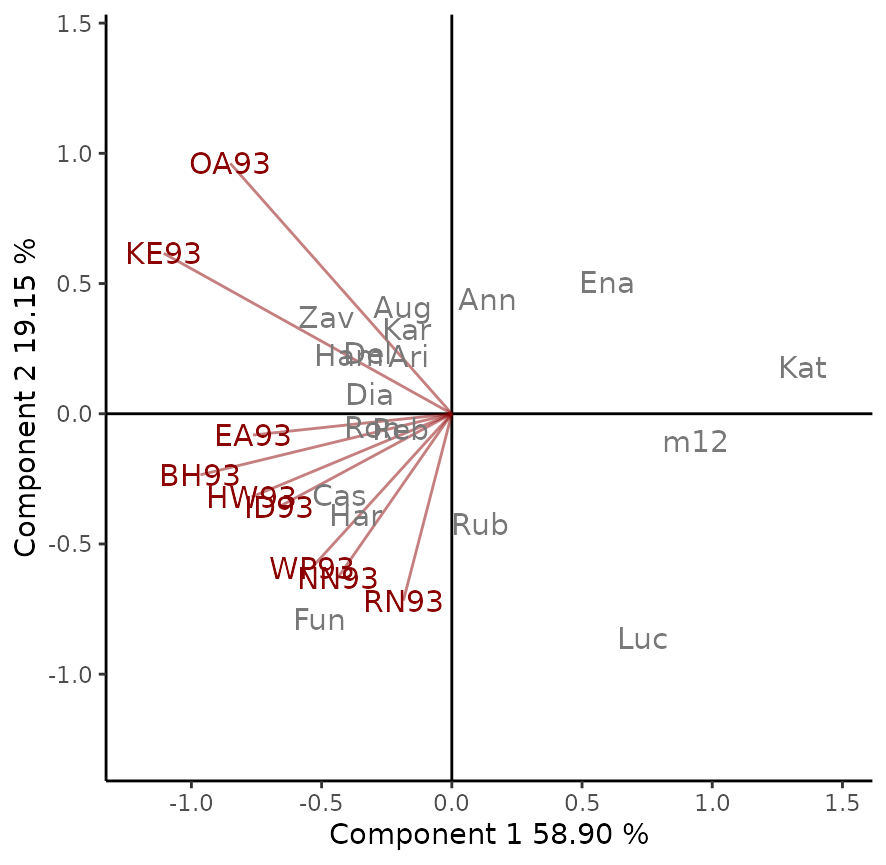
\includegraphics[width=10cm]{./Graficos/GGE_BIPLOT.png}
	\end{center}
	\caption{Biplot básico obtenido de la función \emph{GGEPlot}}
\end{figure}

\item Ranking de los cultivares en función de su rendimiento en el ambiente OA93.

\begin{lstlisting}
GGEPlot(GGE1, type = "Selected Environment", selectedE = "OA93")
\end{lstlisting}


\begin{figure}[h!]
	\begin{center}
		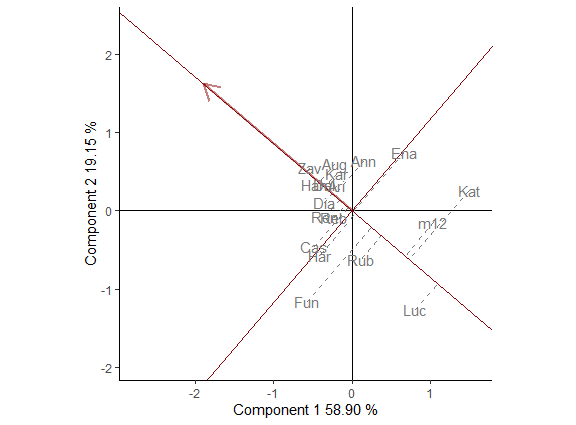
\includegraphics[width=10cm]{./Graficos/SelectedEnvironment.png}
	\end{center}
	\caption{Ranking de cultivares para un ambiente determinado obtenido de la función \emph{GGEPlot}}
\end{figure}


\item Ranking de los ambientes en función del rendimiento relativo del cultivar Kat.

\begin{lstlisting}
GGEPlot(GGE1, type = "Selected Genotype", selectedG = "Kat")
\end{lstlisting}

\begin{figure}[h!]
	\begin{center}
		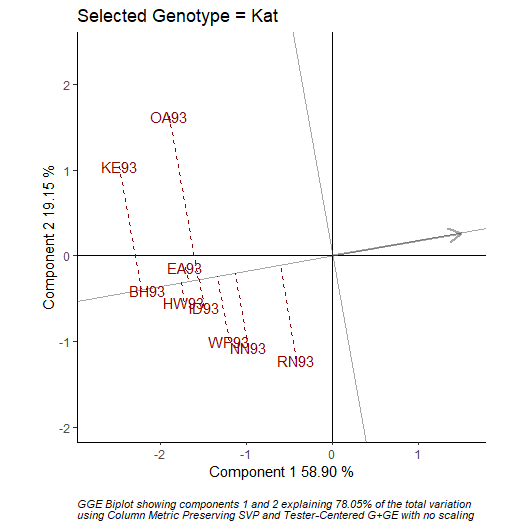
\includegraphics[width=10cm]{./Graficos/SelectedGenotype.png}
	\end{center}
	\caption{Ranking de ambientes para cultivar determinado obtenido de la función \emph{GGEPlot}}
\end{figure}


\item Relación entre ambientes.

\begin{lstlisting}
GGEPlot(GGE1, type = "Relationship Among Environments")
\end{lstlisting}

\begin{figure}[h!]
	\begin{center}
		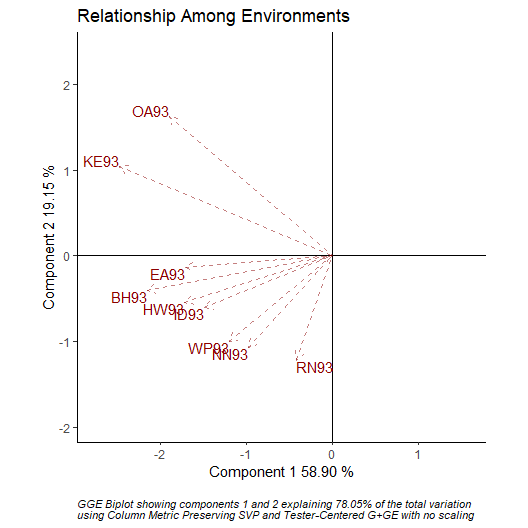
\includegraphics[width=10cm]{./Graficos/RelationshipAmongEnvironments.png}
	\end{center}
	\caption{Relación entre ambientes obtenido de la función \emph{GGEPlot}}
\end{figure}

\item Comparación entre los genotipos Kat y Cas.

\begin{lstlisting}
GGEPlot(GGE1, type = "Comparison of Genotype", selectedG1 = "Kat", selectedG2 = "Cas")
\end{lstlisting}

\begin{figure}[h!]
	\begin{center}
		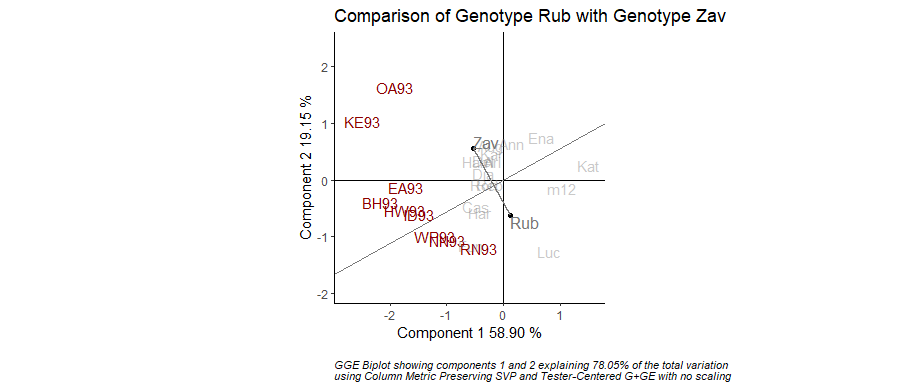
\includegraphics[width=10cm]{./Graficos/ComparisonofGenotype.png}
	\end{center}
	\caption{Comparación entre dos genotipos obtenido de la función \emph{GGEPlot}}
\end{figure}


\item Identificación del mejor cultivar en cada ambiente.

\begin{lstlisting}
GGEPlot(GGE1, type = "Which Won Where/What")
\end{lstlisting}

\begin{figure}[h!]
	\begin{center}
		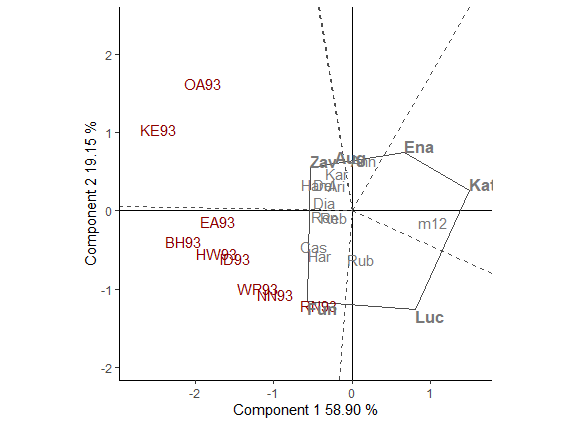
\includegraphics[width=12cm]{./Graficos/WhichWonWhereWhat.png}
	\end{center}
	\caption{Identificación del mejor cultivar en cada ambiente a partir de la función \emph{GGEPlot}}
\end{figure}



\item Evaluación de los ambientes basados tanto en la capacidad de discriminación como en la representatividad.

\begin{lstlisting}
GGEPlot(GGE1, type = "Discrimination vs. representativeness")
\end{lstlisting}

\begin{figure}[h!]
	\begin{center}
		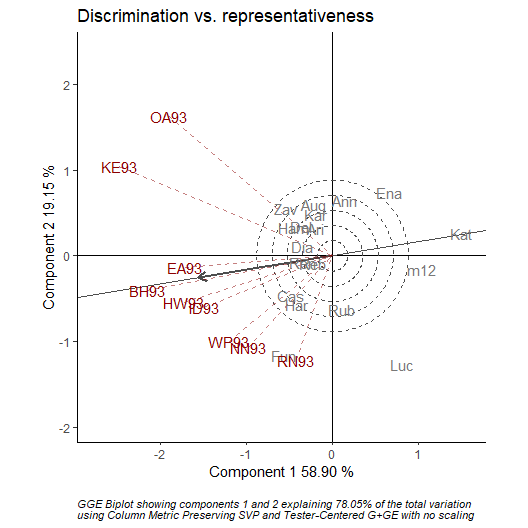
\includegraphics[width=12cm]{./Graficos/Discriminationvsrepresentativeness.png}
	\end{center}
	\caption{Evaluación de los ambientes basados tanto en la capacidad de discriminación y representatividad a partir de la función \emph{GGEPlot}}
\end{figure}



\item Clasificación de ambientes con respecto al ambiente ideal.

\begin{lstlisting}
GGEPlot(GGE1, type = "Ranking Environments")
\end{lstlisting}

\begin{figure}[h!]
	\begin{center}
		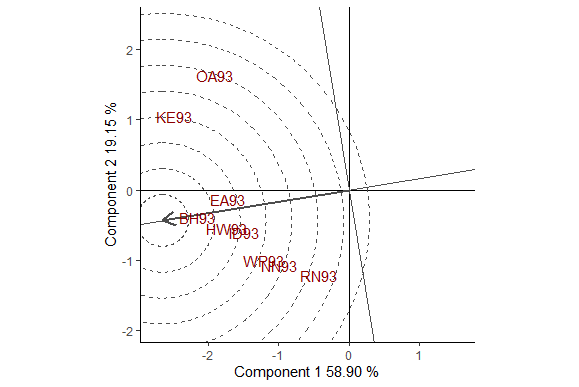
\includegraphics[width=12cm]{./Graficos/RankingEnvironments.png}
	\end{center}
	\caption{Clasificación de ambientes con respecto al ambiente ideal a partir de la función \emph{GGEPlot}}
\end{figure}


\item Clasificación de genotipos con respecto al genotipo ideal.

\begin{lstlisting}
GGEPlot(GGE1, type = "Ranking Genotypes")
\end{lstlisting}

\begin{figure}[h!]
	\begin{center}
		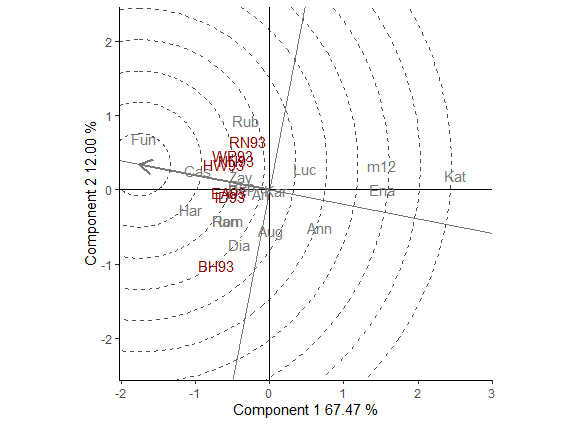
\includegraphics[width=10cm]{./Graficos/RankingGenotypes.png}
	\end{center}
	\caption{Clasificación de genotipos con respecto al genotipo ideal a partir de la función \emph{GGEPlot}}
\end{figure}

\item Evaluación de los cultivares con base en el rendimiento promedio y la estabilidad.

\begin{lstlisting}
GGEPlot(GGE1, type = "Mean vs. Stability")
\end{lstlisting}

\begin{figure}[h!]
	\begin{center}
		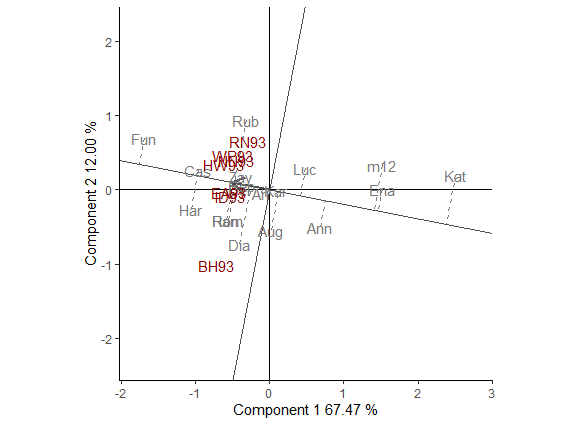
\includegraphics[width=10cm]{./Graficos/MeanvsStability.png}
	\end{center}
	\caption{Evaluación de los cultivares con base en el rendimiento promedio y la estabilidad a partir de la función \emph{GGEPlot}}
\end{figure}

\end{itemize}


\textbf{Classic AMMI model}

Para ejecutar la función rAMMI, como en la función \emph{GGEmodel}, se debe proporcionar un conjunto de datos con genotipo, entorno, repeticiones (si las hay) y la variable de respuesta. Se debe indicar el nombre de las columnas que contienen cada una de estas variables en el conjunto de datos de entradas. La salida de la función es un biplot.

A continuación se muestra el biplot GE obtenido del modelo AMMI clásico obtenido con el conjunto de datos yan.winterwheat.

\begin{lstlisting}
rAMMI(dat_yan, genotype = "gen", environment = "env", response = "yield",
 type = "AMMI")
\end{lstlisting}

\begin{figure}[h!]
	\begin{center}
		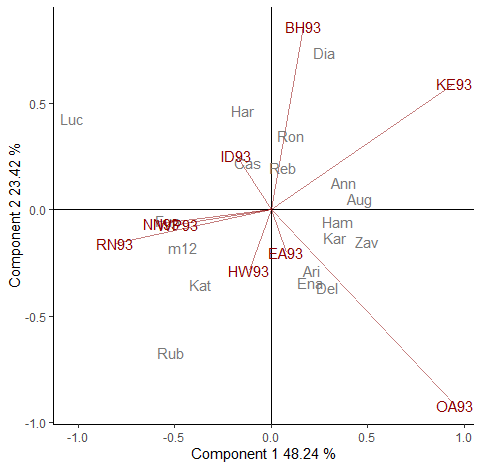
\includegraphics[width=10cm]{./Graficos/AMMI.png}
	\end{center}
	\caption{Biplot GE obtenido del modelo clasico AMMI}
\end{figure}

\textbf{Robust AMMI model}

Como se dijo anteriormente, el modelo AMMI clasico, en su forma estándar, no funciona bien en presencia de observaciones atípicas. Dado que los outliers son muy comun en los datos agronómicos, Rodrigues et al. (2015) proponen cinco modelos AMMI robustos, que permiten superar el problema de la contaminación de datos con observaciones atípicas. Los biplots de los cinco modelos AMMI robustos propuestos por Rodrigues et al. (2015), usando el conjunto de datos yan.winterwheat se muestran a continuación.

\begin{itemize}

\item  modelo "rAMMI"

\begin{lstlisting}
rAMMI(dat_yan, genotype = "gen", environment = "env", response = "yield",
 type = "rAMMI")
\end{lstlisting}

\begin{figure}[h!]
	\begin{center}
		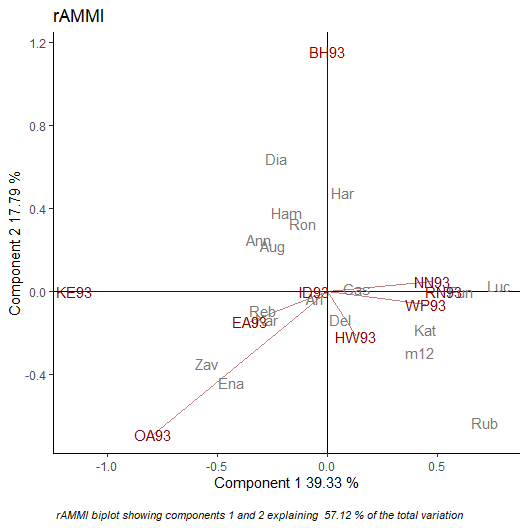
\includegraphics[width=10cm]{./Graficos/rAMMI.png}
	\end{center}
	\caption{Biplot GE obtenido del modelo robusto rAMMI}
\end{figure}


\item  modelo "hAMMI"

\begin{lstlisting}
rAMMI(dat_yan, genotype = "gen", environment = "env", response = "yield",
 type = "hAMMI")
\end{lstlisting}

\begin{figure}[h!]
	\begin{center}
		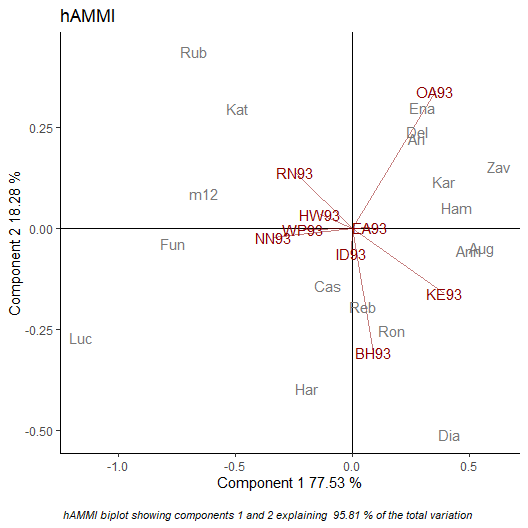
\includegraphics[width=10cm]{./Graficos/hAMMI.png}
	\end{center}
	\caption{Biplot GE obtenido del modelo robusto hAMMI}
\end{figure}


\item  modelo "gAMMI"

\begin{lstlisting}
rAMMI(dat_yan, genotype = "gen", environment = "env", response = "yield",
 type = "gAMMI")
\end{lstlisting}

\begin{figure}[h!]
	\begin{center}
		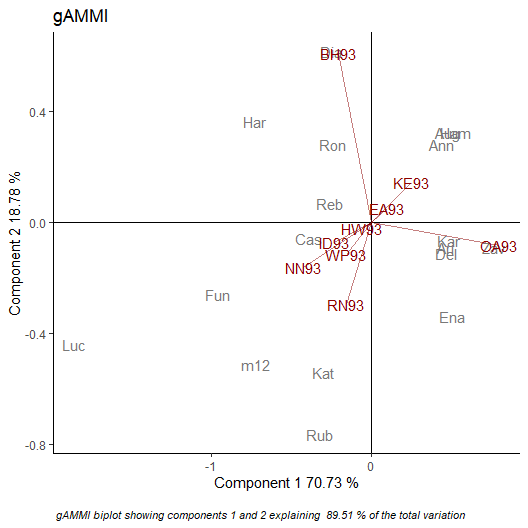
\includegraphics[width=10cm]{./Graficos/gAMMI.png}
	\end{center}
	\caption{Biplot GE obtenido del modelo robusto gAMMI}
\end{figure}



\item  modelo "lAMMI"

\begin{lstlisting}
rAMMI(dat_yan, genotype = "gen", environment = "env", response = "yield",
 type = "lAMMI")
\end{lstlisting}


\begin{figure}[h!]
	\begin{center}
		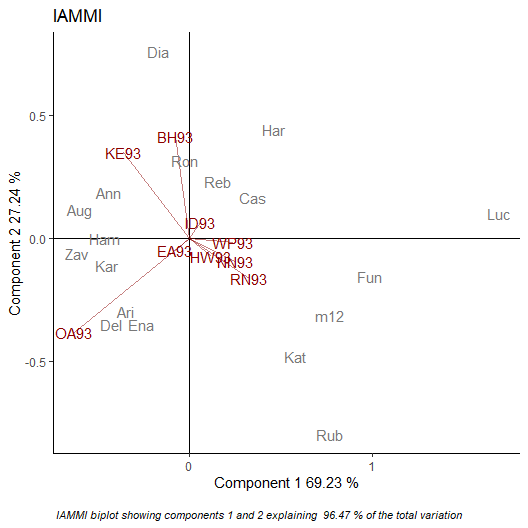
\includegraphics[width=10cm]{./Graficos/lAMMI.png}
	\end{center}
	\caption{Biplot GE obtenido del modelo robusto lAMMI}
\end{figure}


\item  modelo "ppAMMI"
\begin{lstlisting}
rAMMI(dat_yan, genotype = "gen", environment = "env", response = "yield",
 type = "ppAMMI")
\end{lstlisting}


\begin{figure}[h!]
	\begin{center}
		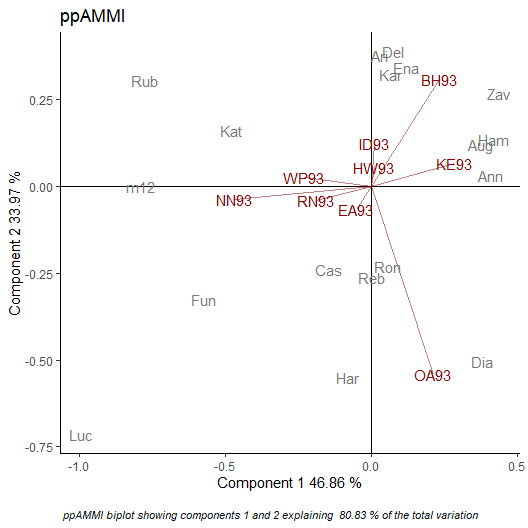
\includegraphics[width=10cm]{./Graficos/ppAMMI.png}
	\end{center}
	\caption{Biplot GE obtenido del modelo robusto ppAMMI}
\end{figure}

\end{itemize}

\textbf{Métodos de imputación}
Una limitación importante de los modelos presentados anteriormente es que requieren una que el conjunto de datos este completo. Por lo tanto, en el paquete se incluyen una serie de metodologías propuestas, algunas de las cuales no se encuentran disponible en R, para superar el problema de falta de equilibrio. 

El conjunto de datos yan.winterwheat se utilizó como ejemplo. Como el conjunto de datos no contaba con observaciones perdidas, algunas fueron eliminadas con el objetivo de mostrar las metodologías de imputación incluidas.

\begin{lstlisting}
# generates missing data
dat_yan[1, 3] <- NA
dat_yan[3, 3] <- NA
dat_yan[2, 3] <- NA
\end{lstlisting}


\begin{itemize}
\item GabrielEigein proposed by Arciniegas-Alarcón S., et al. (2010).
\end{itemize}
\begin{lstlisting}
imputation(dat_yan, PC.nb = 2, genotype = "gen", environment = "env", response = "yield", 
    type = "EM-AMMI")
\end{lstlisting}

\begin{verbatim}
##         BH93  EA93  HW93  ID93  KE93  NN93  OA93  RN93  WP93
## Ann 4.150120 4.150 2.849 3.084 5.940 4.450 4.351 4.039 2.672
## Ari 4.035814 4.771 2.912 3.506 5.699 5.152 4.956 4.386 2.938
## Aug 4.305244 4.578 3.098 3.460 6.070 5.025 4.730 3.900 2.621
## Cas 4.732000 4.745 3.375 3.904 6.224 5.340 4.226 4.893 3.451
## Del 4.390000 4.603 3.511 3.848 5.773 5.421 5.147 4.098 2.832
## Dia 5.178000 4.475 2.990 3.774 6.583 5.045 3.985 4.271 2.776
## Ena 3.375000 4.175 2.741 3.157 5.342 4.267 4.162 4.063 2.032
## Fun 4.852000 4.664 4.425 3.952 5.536 5.832 4.168 5.060 3.574
## Ham 5.038000 4.741 3.508 3.437 5.960 4.859 4.977 4.514 2.859
## Har 5.195000 4.662 3.596 3.759 5.937 5.345 3.895 4.450 3.300
## Kar 4.293000 4.530 2.760 3.422 6.142 5.250 4.856 4.137 3.149
## Kat 3.151000 3.040 2.388 2.350 4.229 4.257 3.384 4.071 2.103
## Luc 4.104000 3.878 2.302 3.718 4.555 5.149 2.596 4.956 2.886
## Reb 4.375000 4.701 3.655 3.592 6.189 5.141 3.933 4.208 2.925
## Ron 4.940000 4.698 2.950 3.898 6.063 5.326 4.302 4.299 3.031
## Rub 3.786000 4.969 3.379 3.353 4.774 5.304 4.322 4.858 3.382
## Zav 4.238000 4.654 3.607 3.914 6.641 4.830 5.014 4.363 3.111
## m12 3.340000 3.854 2.419 2.783 4.629 5.090 3.281 3.918 2.561
\end{verbatim}


\begin{itemize}
\item EM-AMMI proposed by Gauch and Zobel (1990).
\end{itemize}
\begin{lstlisting}
imputation(dat_yan, PC.nb = 1, genotype = "gen", environment = "env", response = "yield", 
    type = "EM-AMMI")
\end{lstlisting}

\begin{verbatim}
##         BH93  EA93  HW93  ID93  KE93  NN93  OA93  RN93  WP93
## Ann 4.136249 4.150 2.849 3.084 5.940 4.450 4.351 4.039 2.672
## Ari 4.474249 4.771 2.912 3.506 5.699 5.152 4.956 4.386 2.938
## Aug 4.386299 4.578 3.098 3.460 6.070 5.025 4.730 3.900 2.621
## Cas 4.732000 4.745 3.375 3.904 6.224 5.340 4.226 4.893 3.451
## Del 4.390000 4.603 3.511 3.848 5.773 5.421 5.147 4.098 2.832
## Dia 5.178000 4.475 2.990 3.774 6.583 5.045 3.985 4.271 2.776
## Ena 3.375000 4.175 2.741 3.157 5.342 4.267 4.162 4.063 2.032
## Fun 4.852000 4.664 4.425 3.952 5.536 5.832 4.168 5.060 3.574
## Ham 5.038000 4.741 3.508 3.437 5.960 4.859 4.977 4.514 2.859
## Har 5.195000 4.662 3.596 3.759 5.937 5.345 3.895 4.450 3.300
## Kar 4.293000 4.530 2.760 3.422 6.142 5.250 4.856 4.137 3.149
## Kat 3.151000 3.040 2.388 2.350 4.229 4.257 3.384 4.071 2.103
## Luc 4.104000 3.878 2.302 3.718 4.555 5.149 2.596 4.956 2.886
## Reb 4.375000 4.701 3.655 3.592 6.189 5.141 3.933 4.208 2.925
## Ron 4.940000 4.698 2.950 3.898 6.063 5.326 4.302 4.299 3.031
## Rub 3.786000 4.969 3.379 3.353 4.774 5.304 4.322 4.858 3.382
## Zav 4.238000 4.654 3.607 3.914 6.641 4.830 5.014 4.363 3.111
## m12 3.340000 3.854 2.419 2.783 4.629 5.090 3.281 3.918 2.561
\end{verbatim}



\begin{itemize}
\item EM-SVD proposed by Perry (2009)
\end{itemize}
\begin{lstlisting}
imputation(dat_yan, genotype = "gen", environment = "env", response = "yield", 
    type = "EM-SVD")
\end{lstlisting}

\begin{verbatim}
##           [,1]  [,2]  [,3]  [,4]  [,5]  [,6]  [,7]  [,8]  [,9]
##  [1,] 4.332467 4.150 2.849 3.084 5.940 4.450 4.351 4.039 2.672
##  [2,] 4.332467 4.771 2.912 3.506 5.699 5.152 4.956 4.386 2.938
##  [3,] 4.332467 4.578 3.098 3.460 6.070 5.025 4.730 3.900 2.621
##  [4,] 4.732000 4.745 3.375 3.904 6.224 5.340 4.226 4.893 3.451
##  [5,] 4.390000 4.603 3.511 3.848 5.773 5.421 5.147 4.098 2.832
##  [6,] 5.178000 4.475 2.990 3.774 6.583 5.045 3.985 4.271 2.776
##  [7,] 3.375000 4.175 2.741 3.157 5.342 4.267 4.162 4.063 2.032
##  [8,] 4.852000 4.664 4.425 3.952 5.536 5.832 4.168 5.060 3.574
##  [9,] 5.038000 4.741 3.508 3.437 5.960 4.859 4.977 4.514 2.859
## [10,] 5.195000 4.662 3.596 3.759 5.937 5.345 3.895 4.450 3.300
## [11,] 4.293000 4.530 2.760 3.422 6.142 5.250 4.856 4.137 3.149
## [12,] 3.151000 3.040 2.388 2.350 4.229 4.257 3.384 4.071 2.103
## [13,] 4.104000 3.878 2.302 3.718 4.555 5.149 2.596 4.956 2.886
## [14,] 4.375000 4.701 3.655 3.592 6.189 5.141 3.933 4.208 2.925
## [15,] 4.940000 4.698 2.950 3.898 6.063 5.326 4.302 4.299 3.031
## [16,] 3.786000 4.969 3.379 3.353 4.774 5.304 4.322 4.858 3.382
## [17,] 4.238000 4.654 3.607 3.914 6.641 4.830 5.014 4.363 3.111
## [18,] 3.340000 3.854 2.419 2.783 4.629 5.090 3.281 3.918 2.561
\end{verbatim}


\begin{itemize}
\item WGabriel proposed by Alarcon…..
\end{itemize}
\begin{lstlisting}
imputation(dat_yan, genotype = "gen", environment = "env", response = "yield", 
    type = "WGabriel")
\end{lstlisting}

\begin{verbatim}
##         BH93  EA93  HW93  ID93  KE93  NN93  OA93  RN93  WP93
## Ann 4.004664 4.150 2.849 3.084 5.940 4.450 4.351 4.039 2.672
## Ari 4.455727 4.771 2.912 3.506 5.699 5.152 4.956 4.386 2.938
## Aug 4.328095 4.578 3.098 3.460 6.070 5.025 4.730 3.900 2.621
## Cas 4.732000 4.745 3.375 3.904 6.224 5.340 4.226 4.893 3.451
## Del 4.390000 4.603 3.511 3.848 5.773 5.421 5.147 4.098 2.832
## Dia 5.178000 4.475 2.990 3.774 6.583 5.045 3.985 4.271 2.776
## Ena 3.375000 4.175 2.741 3.157 5.342 4.267 4.162 4.063 2.032
## Fun 4.852000 4.664 4.425 3.952 5.536 5.832 4.168 5.060 3.574
## Ham 5.038000 4.741 3.508 3.437 5.960 4.859 4.977 4.514 2.859
## Har 5.195000 4.662 3.596 3.759 5.937 5.345 3.895 4.450 3.300
## Kar 4.293000 4.530 2.760 3.422 6.142 5.250 4.856 4.137 3.149
## Kat 3.151000 3.040 2.388 2.350 4.229 4.257 3.384 4.071 2.103
## Luc 4.104000 3.878 2.302 3.718 4.555 5.149 2.596 4.956 2.886
## Reb 4.375000 4.701 3.655 3.592 6.189 5.141 3.933 4.208 2.925
## Ron 4.940000 4.698 2.950 3.898 6.063 5.326 4.302 4.299 3.031
## Rub 3.786000 4.969 3.379 3.353 4.774 5.304 4.322 4.858 3.382
## Zav 4.238000 4.654 3.607 3.914 6.641 4.830 5.014 4.363 3.111
## m12 3.340000 3.854 2.419 2.783 4.629 5.090 3.281 3.918 2.561
\end{verbatim}

\begin{itemize}
\item EM-PCA proposed by
\end{itemize}
\begin{lstlisting}
imputation(dat_yan, genotype = "gen", environment = "env", response = "yield", 
    type = "EM-PCA")
\end{lstlisting}

\begin{verbatim}
##         BH93  EA93  HW93  ID93  KE93  NN93  OA93  RN93  WP93
## Ann 3.980317 4.150 2.849 3.084 5.940 4.450 4.351 4.039 2.672
## Ari 4.463093 4.771 2.912 3.506 5.699 5.152 4.956 4.386 2.938
## Aug 4.327731 4.578 3.098 3.460 6.070 5.025 4.730 3.900 2.621
## Cas 4.732000 4.745 3.375 3.904 6.224 5.340 4.226 4.893 3.451
## Del 4.390000 4.603 3.511 3.848 5.773 5.421 5.147 4.098 2.832
## Dia 5.178000 4.475 2.990 3.774 6.583 5.045 3.985 4.271 2.776
## Ena 3.375000 4.175 2.741 3.157 5.342 4.267 4.162 4.063 2.032
## Fun 4.852000 4.664 4.425 3.952 5.536 5.832 4.168 5.060 3.574
## Ham 5.038000 4.741 3.508 3.437 5.960 4.859 4.977 4.514 2.859
## Har 5.195000 4.662 3.596 3.759 5.937 5.345 3.895 4.450 3.300
## Kar 4.293000 4.530 2.760 3.422 6.142 5.250 4.856 4.137 3.149
## Kat 3.151000 3.040 2.388 2.350 4.229 4.257 3.384 4.071 2.103
## Luc 4.104000 3.878 2.302 3.718 4.555 5.149 2.596 4.956 2.886
## Reb 4.375000 4.701 3.655 3.592 6.189 5.141 3.933 4.208 2.925
## Ron 4.940000 4.698 2.950 3.898 6.063 5.326 4.302 4.299 3.031
## Rub 3.786000 4.969 3.379 3.353 4.774 5.304 4.322 4.858 3.382
## Zav 4.238000 4.654 3.607 3.914 6.641 4.830 5.014 4.363 3.111
## m12 3.340000 3.854 2.419 2.783 4.629 5.090 3.281 3.918 2.561
\end{verbatim}


\section{Geneticae Shiny Web App}

Hoy, los programas de computadora se han convertido en una herramienta básica para el análisis de datos. Actualmente, R es uno de los programas más utilizados debido a su poder y distribución gratuita. R tiene una sintaxis compleja y, por lo tanto, no es del todo amigable para aquellos que no tienen conocimiento del lenguaje de programación R.

Con frecuencia, los mejoradores usan programas que tienen una interfaz para realizar el análisis estadístico deseado y sin necesidad del manejo de un lenguaje de programación. El objetivo de esta aplicación Shiny es crear una interfaz gráfica para eliminar el obstáculo de la complejidad del software para el análisis de los datos provenientes de MET. Geneticae Shiny Web App
es un software interactivo, no comercial y de código abierto, que ofrece una alternativa gratuita al software comercial disponible.

\subsection{Conjuntos de datos en disponibles en Shiny Web App}

La aplicación Shiny Web App cuenta con los dos conjuntos de datos disponibles en el paquete agricolae. Los mismo se pueden descargar con el fin de probar la aplicación. Además, estos son utilizados para desarrollar los ejemplosque se presentan a continuación y en la ayuda disponible en la aplicación.

Los mismos se pueden ver y descargar en la pestaña data $\rightarrow$ Example datasets. 

\begin{figure}[h!]
	\begin{center}
		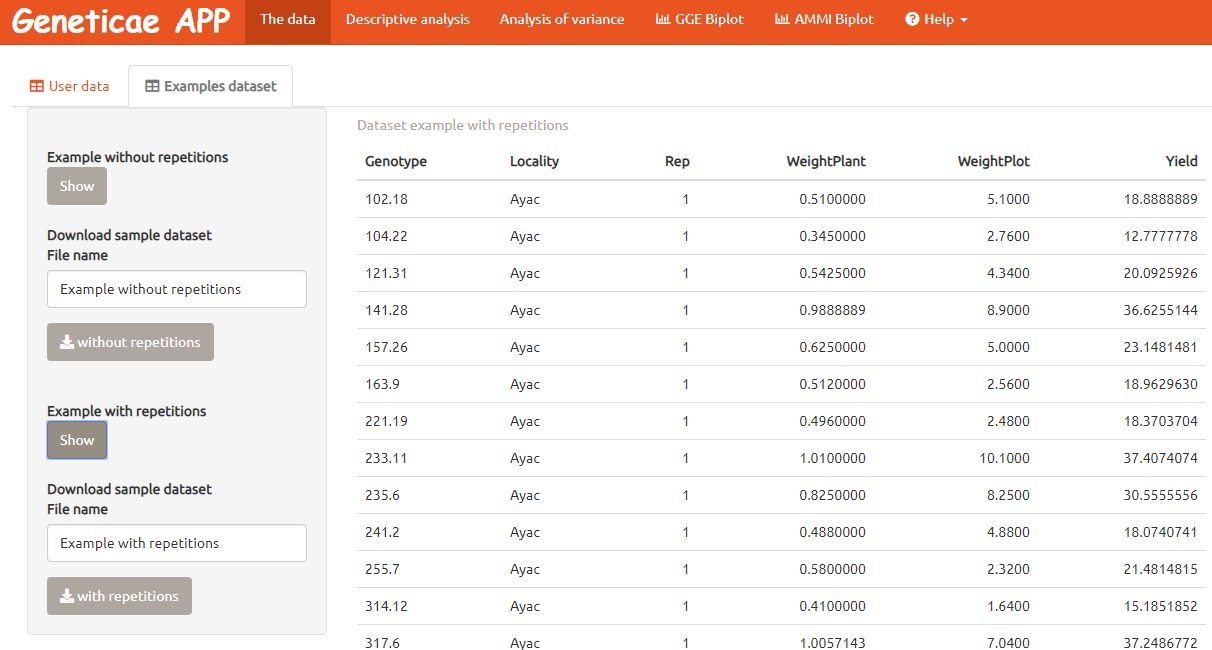
\includegraphics[width=17cm]{./Graficos/Exampledatasets_withoutrep.png}
	\end{center}
	\caption{Conjunto de datos sin repetición disponible en Shiny Web App}
\end{figure}


\begin{figure}[h!]
	\begin{center}
		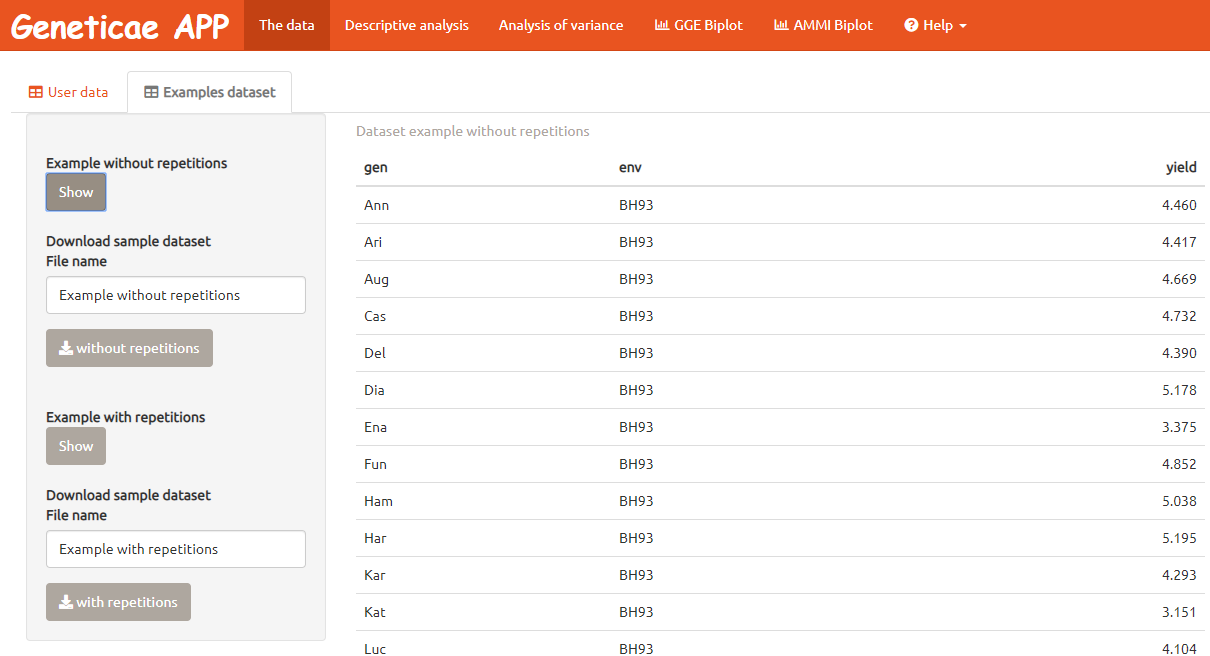
\includegraphics[width=17cm]{./Graficos/Exampledatasets_withrep.png}
	\end{center}
	\caption{Conjunto de datos sin repetición disponible en Shiny Web App}
\end{figure}

\subsection{Análisis disponibles con Shiny Web App}


